\documentclass[12pt]{article}
\usepackage{amsmath}
\usepackage{graphicx}
\graphicspath{ {images/} }
\usepackage{hyperref}
\usepackage[utf8]{inputenc}
\usepackage[backend=biber, style=authoryear, sorting=nty]{biblatex}
\renewcommand*{\nameyeardelim}{\addcomma\space}
\addbibresource{bibliography.bib}

\title{%
  Building a programming language without the dependency on English \\
  \large CMP6102 Individual Project:
 Project Mini-Proposal }

\author{Pandelis Zembashis | S15101590 \\ 
Supervisor: Emmmett Cooper}

\date{October 2018}

\begin{document}
\maketitle

\section{Inspiration}

Computer languages are heavily westernised as the majority of 
early innovation around computer science, in the late 50's to 60's 
took place in the west (North America and Europe). Most if not all
modern programming languages can trace their routes back to two of
most influencial langauges of this time period, ALGOL 68 and COBOL 
\parencite{5396281}. Both of these languages were invented in a time
where all interested parties were English speaking and were inventing
processes that would go on to be used by parties that could communicate
in English at some level. Not to mention that the most common input to this
day is still the qwerty keyboard which is comprised of latin characters.

These early languages have grandfathered in English and the Latin 
character set as the basis for all programming languages we see today. 
This is inreadibly limitting to the creatitivity of a given language,
and the accessibility to non native English speakers or different cultures. 
We have limited ourselves to the symbols available to a character set that was not designed with the intention
to be used to program.

\section{The Idea}

I propose a language be designed around its own character set without the dependency on English at its core.
There are alternate writing systems that use logographic character sets where in which a single
character can describe an entire word or phrase, take Chinese and its derivative script Japanese Kanji or Egyption hieroglyphs for example.
Using this logophraphic system as inspiration for a language opens up many more creative
avenues for how the language can be designed. 

We can assign any meaning we wish to an arbitrary character
instead of taking a complex set of English words or symbols to create language keywords we can have language symbols dedicated to each task.
Similar to how some programming languages allow for macros, a single instruction that expands automatically into a set of instructions to perform a particular task,
we could assign complex behaviour to single symbols.

Take this example of a fizz buzz program in a traditional language like Javascript \ref{fig:javascript} and pseudocode of a made up logophraphic language \ref{fig:logograph}.
In this progrma any numbers divisible by 3 return Fizz, 5 return Buzz and if divisible by both it returns FizzBuzz.

\begin{figure}[h]
    \caption{Example of fizz buzz program in Javascript}
    \centering
    \begin{verbatim}
                for (var i=1; i <= 20; i++)
                {
                    if (i % 15 == 0)
                        console.log("FizzBuzz");
                    else if (i % 3 == 0)
                        console.log("Fizz");
                    else if (i % 5 == 0)
                        console.log("Buzz");
                    else
                        console.log(i);
                }
    \end{verbatim}
    \label{fig:logograph}
\end{figure}    


\begin{figure}[h]
    \caption{Pseudocode example of a logographic approach}
    \centering
    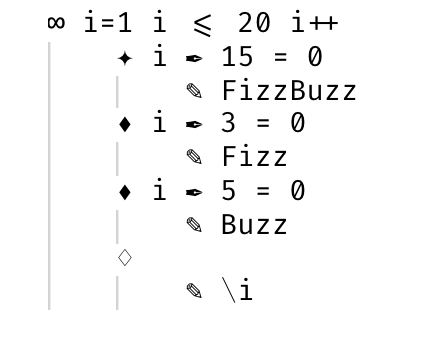
\includegraphics[width=10cm]{logograph}
    \label{fig:javascript}
\end{figure}   


\clearpage

\printbibliography

\end{document}
